\documentclass[12pt,letterpaper]{article}
\usepackage{graphicx,textcomp}
\usepackage{natbib}
\usepackage{setspace}
\usepackage{fullpage}
\usepackage{color}
\usepackage[reqno]{amsmath}
\usepackage{amsthm}
\usepackage{fancyvrb}
\usepackage{amssymb,enumerate}
\usepackage[all]{xy}
\usepackage{endnotes}
\usepackage{lscape}
\newtheorem{com}{Comment}
\usepackage{float}
\usepackage{hyperref}
\newtheorem{lem} {Lemma}
\newtheorem{prop}{Proposition}
\newtheorem{thm}{Theorem}
\newtheorem{defn}{Definition}
\newtheorem{cor}{Corollary}
\newtheorem{obs}{Observation}
\usepackage[compact]{titlesec}
\usepackage{dcolumn}
\usepackage{tikz}
\usetikzlibrary{arrows}
\usepackage{multirow}
\usepackage{xcolor}
\newcolumntype{.}{D{.}{.}{-1}}
\newcolumntype{d}[1]{D{.}{.}{#1}}
\definecolor{light-gray}{gray}{0.65}
\usepackage{url}
\usepackage{listings}
\usepackage{color}
\usepackage[utf8]{inputenc}
\usepackage{verbatim} % includes comment blocks
%\usepackage{rotating}
%\usepackage{geometry}
%\usepackage{pdflscape}
\usepackage{lscape}

\definecolor{codegreen}{rgb}{0,0.6,0}
\definecolor{codegray}{rgb}{0.5,0.5,0.5}
\definecolor{codepurple}{rgb}{0.58,0,0.82}
\definecolor{backcolour}{rgb}{0.95,0.95,0.92}

\lstdefinestyle{mystyle}{
	backgroundcolor=\color{backcolour},
	commentstyle=\color{codegreen},
	keywordstyle=\color{magenta},
	numberstyle=\tiny\color{codegray},
	stringstyle=\color{codepurple},
	basicstyle=\footnotesize,
	breakatwhitespace=false,
	breaklines=true,
	captionpos=b,
	keepspaces=true,
	numbers=left,
	numbersep=5pt,
	showspaces=false,
	showstringspaces=false,
	showtabs=false,
	tabsize=2
}
\lstset{style=mystyle}
\newcommand{\Sref}[1]{Section~\ref{#1}}
\newtheorem{hyp}{Hypothesis}

\title{FUTURE-DATA\\Dublin Bikes}
\date{Due: April 21, 2023}
\author{Ariana Alves Antunes, Imelda Finn, Marcus Ò Faolain}

\begin{document}
	\maketitle
\begin{comment}
\section*{Instructions}
Scenario: You are working for FUTURE-DATA a local company specialised in data science. Dublin City
Council hired your company to study the impact of COVID-19 on the city-bikes usage as they are
planning to optimise the city-bike system. Dublin City Council had originally structured the city-bike
network based on the forecasts of bike usage up to 2030. However, they think that the usage may not
match the initial prediction because of the impact of the pandemic on our mobility. FUTURE-DATA
decided to investigate this rapidly and by formulating multiple scenarios that should be considered by
the City Council. To do so, they assigned the task to k small teams or machine learning and smart and
sustainable cities experts. You are part of one of these k teams.
Task: The company proposed 3 goals. Pick 2 out of the following 3 tasks (two tasks correctly carried
out will give you full points; an extra task will not give any extra points).
1. To assess the impact of the pandemic on the city-bike usage;
2. To estimate how the city-bike usage would have been without the pandemic (e.g., 2020);
3. To predict the city-bike usage for 2022 in both the pandemic and no-pandemic scenarios. Use
both qualitative and quantitative comparisons.
The manager suggested focussing on two or three strategically placed bike stations (of course, you are
free to do more than that, if you like). Make sure that the data for that bike station is available on all
the datasets. Missing or bad data-points can be a problem. So, identifying stations with good data will
make your life easier (but feel free to make your life more complicated if you like the challenge).
Suggestion: The original features tell us about bike and bike stand availability. However, that is a
different concept from “bike usage”. The optimal approach involves deriving a new feature
quantifying the “bike usage” in a given station. Other ways of tackling the tasks are also accepted, but
remember to justify your choices and to plot clear, compact figures


	Submission:
	- A brief report (~2 pages including figures, max 3 pages) with text answering the three
	questions above, and figures (e.g., bar plots) or tables showing the results and data supporting
	your considerations. Remember: You are planning to present this report to your manages AND
	to Dublin City Council. As such, figures must be easy to understand (e.g., large font size, brief
	but meaningful axis labels, include a short caption describing each figure).
	- Your Python scripts. Please write them well, with comments so that I can understand what
	you did. I will use the scripts to double-check your results where necessary.
	- Submission deadline: 21 April 2023.
	- Late submission penalty: 5% * number of days (e.g., 2 days late -> 10% penalty

\end{comment}

\section{Technical/Data issues}
Missing data ...




Picked stations by clustering on ........

Excluded stations with less than 300,000 data points.   None of the stations were open the whole time.
2 stations from each cluster.  The cluster 2 stations had similar pre-pandemic characteristics and both serve hospitals.% Table with station data?, incl stands, colour

\begin{table}[h]
	\centering
	\begin{tabular}{|l|r|r|}
		Station Name & cluster & bike stands\\
		FITZWILLIAM SQUARE EAST & 0 & 40\\
		HANOVER QUAY & 0 & 40\\
		MATER HOSPITAL & 2 & 40\\
		NEW CENTRAL BANK & 1 & 40 \\
		PARNELL SQUARE NORTH & 2 & 20\\
		YORK STREET EAST & 1 & 32 \\
		
	\end{tabular} 
\end{table}


\begin{figure}[!htbp]
	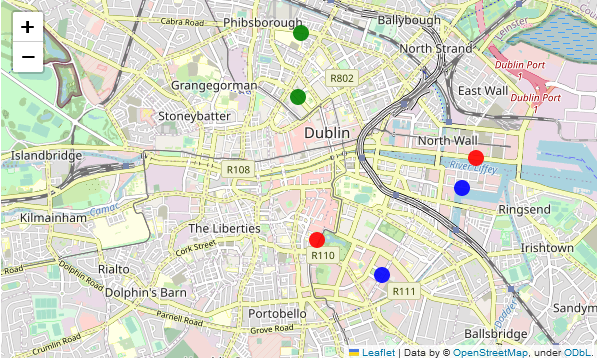
\includegraphics[width=0.7\textwidth]{../graphs/bikeStationMap.png}
	\caption{Selected Bike Stations}
	\label{fig:stations}
\end{figure}

Variable modelled is usage, which is the absolute difference in available bikes from one time point to the next.  For modelling, this is normalised by dividing by the number of bike stands.


\section{The impact of the pandemic on bike usage}
%To assess the impact of the pandemic on the city-bike usage;

\begin{comment}
	\begin{figure}[!htbp]
		\includegraphics[width=0.7\textwidth]{graphs/wireframe.pdf}
		\caption{mle surface}
		\label{fig:surface}
	\end{figure}
	\begin{figure}[!htbp]
		\includegraphics[width=0.7\textwidth]{graphs/q2_xy.png}
		\includegraphics[width=0.7\textwidth]{graphs/q2_hist.png}
		\caption{Q2 Data}
		\label{fig:mle}
	\end{figure}
\end{comment}


\section{Estimated non-pandemic usage for 2020}
%2. To estimate how the city-bike usage would have been without the pandemic (e.g., 2020) 

The bike usage was way down compared to the prediction.\footnote{RidgeCV(alphas=(0.1, 1.0, 10.0), cv=None, fit\_intercept=True, gcv\_mode=None, normalize=False, scoring=None, store\_cv\_values=False)}  
The prediction isn't too bad for January, February, but usage drops at the end of February and stays down for the rest of the year.
\begin{figure}[!htbp]
	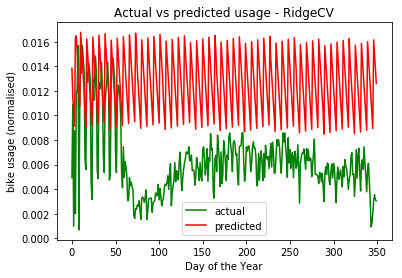
\includegraphics[width=0.7\textwidth]{../graphs/pred_2020.png}
	\caption{Predicted bike usage in 2020, compared to actual usage}
	\label{fig:surface}
\end{figure}


%\section{Predicted bike usage for 2022} 
%To predict the city-bike usage for 2022 in both the pandemic and no-pandemic scenarios. Use both qualitative and quantitative comparisons.

\section*{notes}
\texttt{https://github.com/Arianaxsz/ML-Project}

Code in \texttt{fileName.ipynb}, \texttt{py/fileName.py}


%===============================================================

% # Code snippets

%\vspace{.25cm}
%\noindent  %\href{https://www.researchgate.net/profile/Adam_Przeworski/publication/240357392_Classifying_Political_Regimes/links/0deec532194849aefa000000/Classifying-Political-Regimes.pdf}{Alvarez, Cheibub, Limongi, and Przeworski (1996)}


%\input{tables/zip_poisson.tex}

\begin{comment}
	
	\begin{figure}[!htbp]
		\includegraphics[width=0.7\textwidth]{graphics/wireframe.pdf}
		\caption{mle surface}
		\label{fig:surface}
	\end{figure}
	\begin{figure}[!htbp]
		\includegraphics[width=0.7\textwidth]{graphics/q2_xy.png}
		\includegraphics[width=0.7\textwidth]{graphics/q2_hist.png}
		\caption{Q2 Data}
		\label{fig:mle}
	\end{figure}
\end{comment}

\begin{comment}
	\begin{sidewaystable}
		%\begin{tabular}...\end{tabular}
	\end{sidewaystable}
	%\input{tables/gdp_crosstab.tex}
	
	\begin{landscape}
		\include{tables/gdp_crosstab.tex}
	\end{landscape}
	
\end{comment}


\end{document}
